
%(BEGIN_QUESTION)
% Copyright 2003, Tony R. Kuphaldt, released under the Creative Commons Attribution License (v 1.0)
% This means you may do almost anything with this work of mine, so long as you give me proper credit

A student attempts to build a circuit that will turn a DC motor on and off with a very delicate (low current rating) pushbutton switch.  Unfortunately, there is something wrong with the circuit, because the motor does not turn on no matter what is done with the switch:

$$\includegraphics[width=15.5cm]{i01001x01.eps}$$

Correct the error(s) in this circuit, showing how it must be set up so that the transistor functions as intended.

\underbar{file i01001}
%(END_QUESTION)





%(BEGIN_ANSWER)

$$\includegraphics[width=15.5cm]{i01001x02.eps}$$

%(END_ANSWER)





%(BEGIN_NOTES)


%INDEX% Electronics review, transistor switch circuit (BJT)

%(END_NOTES)


